% -*- TeX -*- -*- Soft -*-
%Daemon> filter=err+warn
%Daemon> custom_args="-synctex=1"
%Daemon> ini=pdflatex

\documentclass{article}
\usepackage{amsmath, amsthm, amssymb}
\usepackage{a4wide}
\usepackage{gamesem}
\usepackage{pst-tree}
%\usepackage{xcolor}
\usepackage{pstring}
\usepackage{todonotes}
\usepackage{amsmath,amssymb,amsthm}

\theoremstyle{definition}
\newtheorem{definition}{Definition}[section]
\newtheorem{remark}{Remark}[section]
\newtheorem{theorem}{Theorem}[section]
\newtheorem{example}{Example}[section]
\newtheorem{observation}{Observation}[section]

\newcommand\Nodes{N}% set of nodes

\newcommand{\ghostlmd}{{\lambda\!\!\lambda}}
\newcommand{\ghostvar}{\theta}

\author{William Blum}
\title{[Draft] On-the-fly eta-expansion for traversing and normalizing ULC terms}

\begin{document}
\maketitle
\begin{abstract}
On-the-fly eta-expanded traversal for the untyped lambda calculus.
(Adapted from the definition used for simply-typed lambda calculus in my thesis \cite{BlumPhd}.)
\end{abstract}

\section{Background}

In \cite{BlumPhd} we establish the correspondence between the theory of traversals and Game semantics for the simply-typed lambda calculus (STLC). The proof in the thesis relies on several ingredients:
\begin{enumerate}
  \item The introduction of a new traversal rule \rulenamet{InputVar} to model free variables;
  \item A formal definition of the notion of \defname{interaction game semantics} corresponding to the game denotation of a term in the usual sense but where internal moves are all revealed instead of hidden;
  \item The definition of various operations on traversals, in particular the notion of \defname{traversal core} which preserves only the ``essence'' of a traversal.
\end{enumerate}


One can then show that, for every simply-typed term $\Gamma \entail M :T$,
there is a bijection $\varphi_M$ from the set of traversals of $M$ to the revealed interaction game denotation of $M$, further there is a bijection between the standard game denotation of $M$ and its standard innocent game denotation. Formally:
\begin{theorem}[STLC Game Semantics and Traversals (Theorem 4.96 in \cite{BlumPhd}]
\label{thm:correspondence}
For every simply-typed term $\Gamma \entail M :T$ there exists two bijections
$\phi_M$ and $\psi_M$:

\begin{eqnarray*}
 \varphi_M  &:& \travset(\Gamma \entail M : T)^\star \stackrel{\cong}{\longrightarrow} \syntrevsem{\Gamma \entail M :T} \\
 \psi_M  &:& \travset(\Gamma \entail M : T)^{\filter \theroot} \stackrel{\cong}{\longrightarrow} \sem{\Gamma \entail M :T} \enspace .
\end{eqnarray*}

where $\syntrevsem{\Gamma \entail M : T}$ denotes the interaction game denotation of $M$, $\sem{\Gamma \entail M : T}$ denotes the innocent game denotation of $M$,
$\travset(M)^\star$ denotes the set of traversals where application nodes are removed, and $\travset(M)^{\filter
\theroot}$ denotes the set of traversal cores of $M$ (\ie traversal projected to the root of the tree).
\end{theorem}

\subsection{Normalizing terms with traversals}

The \defname{projection with respect to the root} of a traversal $t$, noted $t\filter {\theroot}$, gives what we call the \defname{core} of the traversal consisting of the subsequence of nodes that are hereditarily justified by the root. By the correspondence theorem the traversal cores are precisely plays from the game denotation of the term.
Because the traversals P-views (noted $\pview{t}$ for every traversal $t$) correspond to paths in the tree representation of the term (\cite{BlumPhd}, Proposition 4.29), this yields a method to calculate the beta-normal form of any STLC term $M$:
\begin{enumerate}
  \item Enumerate traversals of $M$;
  \item For each traversal $t$, calculate its traversal core $t \filter \theroot$. This gives a play in $\sem{M}$;
  \item Calculate the P-view of the traversal core: $\pview{t\filter \theroot}$;
  \item Apply the Correspondence bijection to get the corresponding path in the tree representation of the $\beta$-nf of $M$.
\end{enumerate}


\begin{remark}
All the traversal rules are deterministic except \rulenamet{InputVar}. The rule \rulenamet{InputVar} gives two non-deterministic choices: (i) the variable to pick in the O-view,
(ii) the child lambda node to pick amongst the picked variable's children.
A consequence of this definition is that even for terms having a normal form (and in particular even for beta-normal terms), the set of traversals can be infinite, and traversals can be infinitely long.
E.g. Take the term $\lambda f . f (\lambda x. x)$. We have that $\lambda f \cdot f \cdot (\lambda x \cdot  x)^k$ is a traversal for all $k\geq0$. Viewed from a game semantic perspective, those traversals accounts for all the possible denotations of the function parameter $f$: observe that for each $k$, there exists a term that applies its argument $k$ times: $\lambda y . y (y ( \ldots y)) $.

\todo{Type my handwritten notes with proof explaining this in more details.}
For the sake of computing the beta-normal form of a term, however, it's only necessary to traverse finitely many finite traversals (provided that the normal form exists). Effectively, this means limiting the rule \rulenamet{InputVar} so that it traverse only nodes leading to paths in the computation tree that are yet unexplored. In practice, it means that when choosing the next lambda node to visit, one can ignore nodes that are already present in the O-view.
\end{remark}

\textbf{Implementation}
This reduction method was implemented in the HOG tool mentioned in my thesis which lets you ``play the traversal game'' and calculate various types of projections including the one giving the traversal cores.

\todo{Cite Neil's paper and discussion.}
The question addressed in the present note is: can this method be extended to the untyped lambda calculus (ULC) following the same game-semantic argument but based on Ker's game model of the untyped lambda calculus instead of the game model of STLC?


\section{Definition}

For an untyped lambda term $M$ we defined its \defname{computation tree} $\tau(M)$ the same way as for the STLC
except that we don't perform eta-long expansion. Consecutive lambda abstractions are still merged into a single nodes in the tree so as to maintain the alternation between lambda nodes (at odd level) and variable nodes (at even level).
Let $\Nodes$ be the set of nodes of the computation tree. We write $\Nodes_{\sf var}$ for the set of variable nodes, $\Nodes_{\sf \lambda}$ for lambda nodes, and $\Nodes_{@}$ for the application nodes.

We defined the \defname{arity} of a node as follows: the arity of a lambda node $\lambda x_1 \cdots x_k$ for $k\geq 0$ is denoted by $|\lambda x_1 \cdots x_k|$ and is defined as $k$; the arity of a variable node $x$, denoted $|x|$ is the number of children of $x$ in the computation tree; the arity of a $@$ node is the number of its children nodes minus 1.

The set $\travset(M)$ of \defname{traversals} over an untyped lambda term $\tau(M)$ is a sequence of elements in $\Nodes + \{ \ghostlmd, \ghostvar \}$ with associated pointers. It is defined by induction over the rules of Table \ref{tab:trav_rules}.
Elements in $N$ represent occurrences of nodes from the original term tree while $\ghostlmd$ and $\ghostvar$ are placeholders representing eta-expanded ``ghost'' lambda nodes and ``ghost'' variable nodes respectively.
By convention ghost variables and lambda nodes are given arity $0$.

A traversal that cannot be extended by any rule is said to be \emph{maximal}.

Note that those rules closely match those of \cite{BlumPhd} for STLC. In the present setting of ULC, however, there are no interpreted constants therefore we don't need the rules \rulenamet{Value} and \rulenamet{InputValue} from the original presentation.

We now fix an untyped term and abbreviated its set of traversals as just $\travset$.

\begin{FramedTable}
\noindent {\bf Structural rules}
\begin{itemize}[]
\item\rulenamet{Root} The singleton sequence $r$ is in $\travset$ where $r$ is the root of the tree.
\end{itemize}

\begin{itemize}[]
    \item \rulenamet{Lam} If $t \cdot \lambda \overline{\xi}$ is a traversal then so is
        $t \cdot \lambda \overline{\xi} \cdot n$ where $n$
        denotes $\lambda \overline{\xi}$'s child in $\tau(M)$ and its justifier is defined as follows. If $n$ is
        \begin{compactitem}
            \item an $@$-node then it has no justifier
            \item in $\Nodes_{\sf fv}$ then it points
            to the only occurrence of the root in
            $\pview{t \cdot \lambda \overline{\xi}}$
            \item in $\Nodes_{\sf var}$ but not in $\Nodes_{\sf fv}$ then it points to the only occurrence of its binder in
            $\pview{t\cdot \lambda \overline{\xi}}$.
        \end{compactitem}
    \item \rulenamet{Lam^\ghostlmd} If
  $\Pstr[0.5cm]{ t \cdot(l){l} \cdot
(v){v} \cdot \ldots \cdot
(gl-v,40:i){\ghostlmd} \in\travset}$ for some prefix $t$, $l\in \Nodes_\lambda + \{\ghostlmd \}$ and $v\in\Nodes_{\sf var} + \{\ghostvar\}$ then
$$\Pstr[0.5cm]{ t \cdot(l){l} \cdot
(v){v}
\cdot \ldots \cdot
(gl-v,40:i){\ghostlmd}\cdot (al-l,40:j){\ghostvar}
     \in\travset}$$
 where $j = |l| + i - |v|$. The placeholder $\ghostvar$ represents an occurrence of the $j$th variable that would be bound by lambda node $l$ if the sub-term at node $l$ were eta-expanded $i-|v|$ times.


    \item \rulenamet{App} If $t \cdot @$ is a traversal then so is \Pstr[0.4cm]{t \cdot (m) @  \cdot (n-m,40:0) n}.
\end{itemize}

\emph{\bf Data - Input-variable rules}

If $t \cdot x$ is a traversal where $x \in \Nodes_{\sf var} + \{\ghostvar \}$ is hereditarily justified by the root:
\begin{itemize}[]
\item \rulenamet{InputVar} If $x\in \Nodes_{\sf var}$ then
$t \cdot x \cdot l \in \travset$ for every
occurrence $v \in \Nodes_{\sf var}$ in $\oview{t\cdot x}$ and every $k$th child $l \in \Nodes_\lambda$ of $v$, where $l$ points to $v$ with label $k$.

\item \rulenamet{InputVar^\eta} If $x\not \in \Nodes_{\sf var}$ (i.e., $x$ is a ghost variable), then $t \cdot x \cdot \ghostlmd \in\travset$ where $\ghostlmd$ points to $\ghostvar$ for every other occurrence $\ghostvar$ in $\oview{t\cdot x}$ and every label $k\geq 1$
    .
\end{itemize}

\emph{\bf Program - Copy-cat rules \underline{with on-the-fly eta-expansion}}

Suppose \Pstr[0.5cm]{t \cdot(l){l} \cdot (n){n} \cdot (lx){\lambda \overline{x} }
    \ldots (x-lx,50:i){x_i} \in \travset} where $i>0$, $x_i \in \Nodes_{\sf var} + \{ \ghostvar\}$ hereditarily justified by an $@$-node; $n \in (\Nodes_{\sf var} \Union \Nodes_{@}) + \{ \ghostvar \}$; and $l \in \Nodes_\lambda + \{\ghostlmd\}$. Then:

\begin{itemize}
  \item \rulenamet{Var} (No expansion) If $i \leq |n|$ then
  $$\Pstr[0.5cm]{ t \cdot(l){l} \cdot
(n){n} \cdot (lx){\lambda \overline{x}}  \ldots (x-lx,30:i){x_i}
    \cdot (letai-n,40:i){\lambda \overline{\eta_i}}
     \in\travset}$$
where $\lambda \overline{\eta_i} \in N$ is the $i$th child of $n$ (which is necessarily a node of the tree since $|n|\geq|i|>0$).

\item \rulenamet{Var^\eta} (Eta-Expansion) If $i > |n|$ then
  $$\Pstr[0.5cm]{ t \cdot(l){l} \cdot
(n){n} \cdot (lx){\lambda \overline{x}}  \ldots (x-lx,30:i){x_i}
    \cdot (letai-n,40:i){\ghostlmd}
     \in\travset}$$
     where the ghost node $\ghostlmd$ represents the $i$th ghost child of $n$.
\end{itemize}

\caption{Traversal rules for the untyped lambda calculus.}
 \label{tab:trav_rules}
\end{FramedTable}

\begin{remark}
The rule \rulenamet{Lam} is well defined. In particular it can be show as in STLC, that P-views are paths in the (possibly eta-expanded) tree thus $n$'s enabler occurs exactly once in the P-view.
\end{remark}

\section{Correspondence}
Following the STLC framework of my thesis, the rule \rulenamet{InputVar} is defined so as to obtain the correspondence with game semantics: the nodes visited by this rule correspond to moves played by the Opponent in the game denotation. (We recall that in Game Semantics, the Opponent represents the environment of the program, or equivalently, the data passed to the program.
We aim to prove that this presentation yields an isomorphism between the set of traversals and the revealed game semantics of the ULC term, and subsequently that it yields an isomorphism between the standard game semantics and the set of traversal cores (i.e., projected wrt. the root):

\begin{theorem}[Correspondence with Game Semantics]
\label{thm:ulc_corresp}
The traversal-game semantics isomoprhism of \cite{BlumPhd} for STLC also yields for ULC using traversal definition from Table \ref{tab:trav_rules} and the game model of ULC from Ker's thesis.
\end{theorem}
\begin{proof}
\todo{add proof sketch!}
Should follow the same argument as \cite{BlumPhd} but using the Ker's game model of ULC instead of the innocent game model of the STLC.
The ``on-the-fly'' eta-expansion should correspond to the $Fun$ morphism of Ker's game category.
\end{proof}

\section{Traversals for normalizing ULC term}

\begin{remark}[Traversals for normalizing term]
The beta-normal form of a term $M$ can be reconstructed from the set of paths in its computation tree. And the set of paths in the computation tree of a beta-normal term is given by the set of P-views of its traversals. Furthermore by the Traversal-Game Semantics isomorphism the set of traversals of the beta-nf is just the set of projection, with respect to the root, of the set of traversal of the $M$ \cite{BlumPhd}.
\end{remark}

\begin{observation}[Finite traversals are enough]
For the purpose of computing beta normal form, the value $k$ in rule $\rulename{InputVar^\eta}$ can be bounded by a computable quantity called the \defname{arity threshold} of the traversal at that point.
\end{observation}

\begin{definition}[Traversal arity threshold]
\label{dfn:arity-threshold}
Take a traversal $t$ where rule $\rulename{InputVar^\eta}$ can be applied. Its \defname{arity threshold} is defined as:
    \begin{align*}
    \textsf{arth}(t) &= \max_{(l,n)\in X(t_0)} |n| - |l| \\
    X(t_0) &= \{ (l,n) \in \Nodes_\lambda \times \Nodes_{\sf var} | \mbox{ $l$ and $n$ occur subsequently in $t_0$ between $\jp(t_0^\omega)$ and $t^\omega$} \}
    \end{align*}
where $t^\omega$ denotes the last occurrence in traversal $t$ and $\jp(t)$ denotes the prefix of $t$ ending at the justifier of the last node of $t$.
\todo{Add notes explaining the idea behind this definition}
\end{definition}

\begin{example}[Walking example ``${\sf add}\ 1$'']
We demonstrate here on a small example, how the beta-normal form of a term can be obtained with traversals.
Consider the Church numerals written $k = \lambda s z . s^k z$ for $k\geq0$. We consider a term $M$ representing the function that adds $1$ to the input integer: $M k$ reduces to $(k+1)$ for all $k$. Such term can be defined as $M \equiv{\sf add}\ 1$ where
${\sf add} \equiv \lambda x y s z. x\, s (y\, s\, z)$.
Note that $M$ is not beta-normal.
The computation tree $\tau(M)$ of $M$ is:
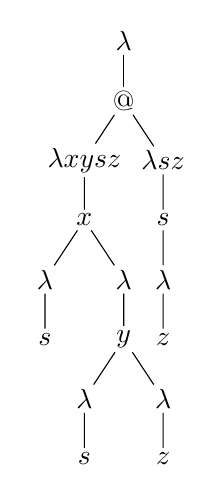
\begin{tikzpicture}[baseline=(root.base),level distance=5ex,inner ysep=0.5mm,sibling distance=10mm]
\node (root)
{$\lambda$}
child {node{$@$}
    child{node{$\lambda x y s z$}
        child { node{$x$}
            child{node{$\lambda$}{
                child {node {$s$}}}
            }
            child{node{$\lambda$}
                child{node{$y$}
                    child{node{$\lambda$}
                        child{ node {$s$}}
                    }
                    child{node{$\lambda$}
                        child{node{$z$}}}
                }
            }
        }
    }
    child{node{$\lambda s z$}
        child{node{$s$}
            child{node{$\lambda$} child{node{$z$}}}
        }
    }
}
;
\end{tikzpicture}

\begin{itemize}
\item Applying as many deterministic rules as possible gives the following traversal at which point the Opponent must make a choice:

$t_0 = \Pstr[0.7cm]{(n0){\lambda }\ (n1){@}\ (n2-n1){\lambda x y s z}\ (n3-n2){x}\ (n4-n1){\lambda s z}\ (n5-n4){s}\ (n6-n3){\lambda }\ (n7-n2){s}\ (n8-n1){\ghostlmd^3}\ (n9-n0){\ghostvar^2} }$

(For readability we indicate the link label in exponent of the source node when representing traversals.)
The core of $t_1$ is
$t_0\filter\theroot = \Pstr[0.7cm]{(n0){\lambda } \cdot (n9-n0){{\ghostvar^2}} }$
and therefore $\pview{t\filter\theroot} =  \lambda \cdot \ghostvar^2$ is a path in  $\betanf{M}$.
This means that $\betanf{M}$ must be of the form $\lambda y s \ldots \cdot y N_1 \ldots \ldots N_q$ for some fresh variable $y$ and $s$ and $q\geq0$.

\item In order to determine what each argument $N_k$ is in the final normal form, we apply the $\rulename{InputVar^\eta}$ rule for each possible argument index $k\geq 0$ and then continue applying the traversal rules.

For $k=1$ we get the traversal:

$t_1 = \Pstr[0.7cm]{(n0){\lambda }\ (n1){@}\ (n2-n1){\lambda x y s z}\ (n3-n2){x}\ (n4-n1){\lambda s z}\
(n5-n4){s}\ (n6-n3){\lambda }\
(n7-n2){s}\ (n8-n1){\ghostlmd^3}\
(n9-n0){\ghostvar^2}
(n10-n9){\ghostlmd^1}
(n11-n8){\ghostvar^1}
(n12-n7){\ghostlmd^1}
(n13-n6){\ghostvar^1}
(n14-n5){\lambda^1}
(n15-n4)z
(n16-n3){\lambda^2}
(n17-n2)y
(n18-n1){\ghostlmd^2}
(n19-n0){\ghostvar^1}
}$

The P-view of the traversal core is
$\pview{t_1\filter\theroot} = \Pstr[0.7cm]{(l){\lambda } \cdot (x-l){\ghostvar^2} \cdot (l1-x){\ghostlmd^1}
\cdot (x2-l){\ghostvar^1}
}$
which means that the normal form is of the form $\lambda y s \ldots \cdot s (y R_1 \ldots R_{q_2}) N_2 \ldots N_q$ for some terms $R_1$, \ldots $R_{q_2}$, and $q,q_2\geq 0$.

\item What should be the value of $q$? In other words, how many more $k$ do we need to look at?  The answer: we need to keep iterating on $k$ until the point where applying the traversal rules will only produce ghost variables and ghost lambda-nodes! Because there is a finite number of nodes in the computation tree, the variable node arities are bounded. Therefore for high enough argument indices $k$, the condition $i\leq|n|$     in the definition of \rulenamet{Var} will never be met:
        after applying rule \rulenamet{InputVar^\eta} on $t_0$, all subsequent extensions of the traversal will be done using either rule $\rulename{Var^\eta}$ or rule $\rulename{Lam^\eta}$.
     The upper-bound $q$ for $k$ is precisely given by the \emph{arity threshold} of the traversal $t_0$ as defined in \ref{dfn:arity-threshold}.
     Here we have ${\sf arth}(t_0) = 1$. Thus we don't need to look at higher value of $k$ and we have:
     $\betanf{M} = \lambda y s \ldots \cdot s (y R_1 \ldots R_{q_2})$.

\item The arity threshold of $t_1$ is ${\sf arth}(t_1) = |\lambda xysz| - |x| = 4 -2 = 2$ hence
    $\betanf{M} = \lambda y s \ldots \cdot s (y R_1 R_2)$.

\item Let's apply the rule \rulenamet{InputVar^\eta} for varying value of child index $1\leq k_2 \leq q_2 = 2$. We first look at the case $k_2 = 1$. The traversal obtained is:

$t_2 = \Pstr[0.7cm]{
(n0){\lambda }\
(n1){@}\ (n2-n1){\lambda x y s z}\ (n3-n2){x}\ (n4-n1){\lambda s z}\ (n5-n4){s}\ (n6-n3){\lambda }\ (n7-n2){s}\ (n8-n1){\ghostlmd^3}\ (n9-n0){\ghostvar^2}
(n10-n9){\ghostlmd^1}
(n11-n8){\ghostvar^1}
(n12-n7){\ghostlmd^1}
(n13-n6){\ghostvar^1}
(n14-n5){\lambda^1}
(n15-n4)z
(n16-n3){\lambda^2}
(n17-n2)y
(n18-n1){\ghostlmd^2}
(n19-n0){\ghostvar^1}
(n20-n19){\ghostlmd^1}
(n21-n18){\ghostvar^1}
(n22-n17,60:1)\lambda % points to non-ghost node
(n23-n2,45:3) s
(n24-n1,45:3) {\ghostlmd^3}
(n25-n0,48:2) {\ghostvar^2}
}$

Thus $\pview{t_2 \filter\theroot} =
\Pstr[0.7cm]{
(n0){\lambda }\
 (n9-n0){\ghostvar^2}
 (n10-n9){\ghostlmd^1}
(n19-n0){\ghostvar^1}
(n20-n19){\ghostlmd^1}
(n25-n0,48:2){\ghostvar^2}
}$

Hence $\betanf{M}$ is of the form $\lambda y s \ldots \cdot s\ (y\ s\ R_2)$.

\item Now let's extend $t_1$ with \rulenamet{InputVar^\lambda} for $k_2 = 2$. We get the traversal:

$t_3 = \Pstr[0.7cm]{
(n0){\lambda }\
(n1){@}\ (n2-n1){\lambda x y s z}\
(n3-n2){x}\ (n4-n1){\lambda s z}\
(n5-n4){s}\
(n6-n3){\lambda }\
(n7-n2){s}\
(n8-n1){\ghostlmd^3}\
(n9-n0) {\ghostvar^2}
(n10-n9) {\ghostlmd^1}
(n11-n8){\ghostvar^1}
(n12-n7){\ghostlmd^1}
(n13-n6){\ghostvar^1}
(n14-n5)\lambda^1
(n15-n4)z
(n16-n3){\lambda^2}
(n17-n2)y
(n18-n1){\ghostlmd^2}
(n19-n0){\ghostvar^1}
(n20-n19){\ghostlmd^2} %%%%%%%%
(n21-n18){\ghostvar^2}
(n22-n17,60:2)\lambda % points to non-ghost node
(n23-n2,45:4) z
(n24-n1,45:4) {\ghostlmd^4}
(n25-n0,48:3) {\ghostvar^3}
}$

Thus $\pview{t_3 \filter\theroot} =
\Pstr[0.7cm]{
(n0){\lambda }\
 (n9-n0){{\ghostvar^2}}
 (n10-n9){\ghostlmd^1}
(n19-n0){\ghostvar^1}
(n20-n19){\ghostlmd^2}
(n25-n0,48:3) {\ghostvar^3}
}$

Hence $\betanf{M} = \lambda y s z \cdot s\ (y\ s\ z)$.
\end{itemize}
\end{example}

\begin{example}[Baby example]
  Take $M = (\lambda x. x x) (\lambda y. y)$.

  $t = \Pstr[0.7cm]{(n0){\lambda }\ (n1){@}\ (n2-n1){\lambda x}\ (n3-n2){x}\ (n4-n1){\lambda y}\ (n5-n4){y}\ (n6-n3){\lambda }\ (n7-n2){x}\ (n8-n1){\lambda y}\ (n9-n8){y}\ (n10-n7){\ghostlmd^1}\ (n11-n6){\ghostvar^1}\ (n12-n5){\ghostlmd^{1}}\ (n13-n4){\ghostvar^2}\ (n14-n3){\ghostlmd^2}\ (n15-n2){\ghostvar^2}\ (n16-n1){\ghostlmd^2}\ (n17-n0){\ghostvar^1}}$

We have $\pview{t\filter\theroot} = \Pstr[0.7cm]{(n0){\lambda }\ (n17-n0){\ghostvar^1}}$
and the traversal arity threshold is $arth(t) = 1$ therefore the beta-normal form of $M$ is $\lambda y . y$.
\end{example}

\begin{example}[Traversals for $varity\ 2$]
\todo{Add traversals for $varity 2$ example.}
\end{example}
\bibliographystyle{abbrv}
\bibliography{ulctrav}

\end{document}
